\chapter{Polarización eléctrica. Condensadores}
\chaptermark{Polarización eléctrica}


\begin{miparrafo}
Un \emph{condensador} o capacitor es un dispositivo que almacena energía potencial eléctrica y carga eléctrica. Para hacer un conensador, basta aislar dos conductores uno del otro. Para almacenar energía en este dispositivo hay que transferir carga de un conductor al otro, de manera que uno tenga carga negativa y en el otro haya una cantidad igual de carga positiva. Debe realizarse trabajo para trasladar las cargas a través de la diferencia de potencial resultante entre los conductores, y el trabajo efectuado se almacena como energía potencial eléctrica. 

Para un condensador en particular, la razón entre la carga de cada conductor y la diferencia de potencial entre los conductores es una constante llamada \emph{capacitancia}. La capacitancia depende de las dimensiones y las formas de los conductores y del material aislante (si lo hay) entre ellos. En comparación con el caso en que sólo hay vacío entre los conductores, la capacitancia aumenta cuando está presente un material aislante (un dieléctrico). Esto sucede porque en el interior del material aislante ocurre una redistribución de la carga, llamada \emph{polarización}. El estudio de la polarización ampliará nuestra perspectiva de las propiedades eléctricas de la materia. 

Los capacitores también ofrecen una forma nueva de pensar acerca de la energía potencial eléctrica. La energía almacenada en un capacitor con carga, guarda relación con el campo eléctrico en el espacio entre los conductores. Veremos que la energía potencial eléctrica puede considerarse almacenada en el mismo campo. La idea de que el campo eléctrico es en sí un almacén de energía está en el corazón de la teoría de las ondas electromagnéticas y de nuestra concepción moderna de la naturaleza de la luz. 	
\end{miparrafo}


\section{Dipolo eléctrico}

Por definición, se dice que un \emph{dipolo eléctrico} está constituido por dos cargas $\pm q$, del mimo valor absoluto y distinto signo separadas una pequeña distancia $a$. Se define el vector $\vec a$ como aquel que une ambas cargas en el sentido  de la carga $-q$ hacia la carga $+q$. Llamaremos \emph{momento dipolar} a

\begin{figure}[H]
	\centering
	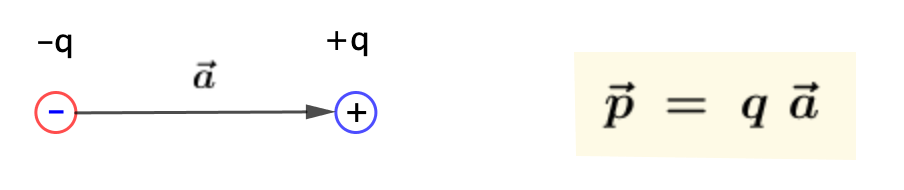
\includegraphics[width=.8\textwidth]{imagenes/imagenes24/T24IM01.png}
\end{figure}

Vamos a calcular el campo y potencial eléctrico de este dipolo a una distancia $r>>a$.


\begin{multicols}{2}
En $A,\ V=V_1+v_2$

$V=\dfrac {q}{4\pi \varepsilon_0 r_1}-{q}{4\pi \varepsilon_0 r_2}$

$V={q}{4\pi \varepsilon_0}\left( \dfrac 1 {r_1} - \dfrac 1 {r_2} \right)$

$V=\dfrac{q}{4\pi \varepsilon_0} \dfrac{r_2-r_1}{r_1r_2}$

Para $r>>a$,
\begin{figure}[H]
	\centering
	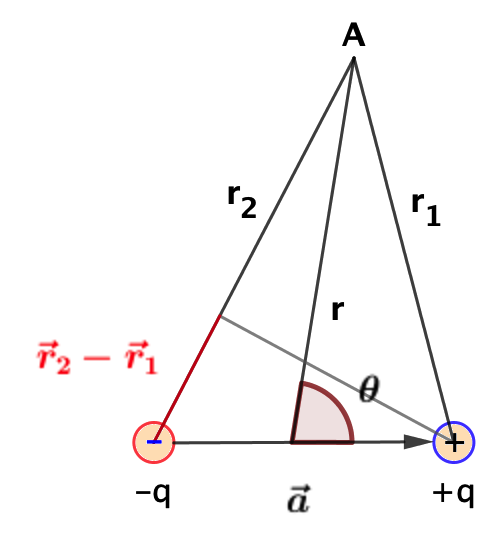
\includegraphics[width=.25\textwidth]{imagenes/imagenes24/T24IM02.png}
\end{figure}	
\end{multicols}

$r>>a \to r_2 \approx r_1; \quad r_2-r_1=a\cos \theta ;\quad r_2r_1=r^2$

$V=\dfrac{q}{4\pi \varepsilon_0} \dfrac {a\cos\theta}{r^2}$; como $p=qa$, tendremos

\begin{equation}
\subrayado{ \ \boxed{ \ 	\boldsymbol{V\ =\ \dfrac{p\ \cos \theta}{4\pi \varepsilon_0\ r^2}} \ } \ } \qquad V=V(p, \theta, r)
\end{equation}

Calculo del campo eléctrico: $\quad \overrightarrow E=- \overrightarrow{\grad} V$

Recordemos la expresión del operador nabla en coordenadas esféricas cuando solo hay dos términos $r$ y $\theta$ ($\varphi$ no afecta).

$\displaystyle \vec u_r E_r+\vec u_\theta E_\theta =-\vec u_r \pdv{V}{r} -\vec u_\theta \dfrac 1 r \pdv{V}{r}$

$\displaystyle E_r=-\pdv{V}{r}= +\dfrac{2p\cos \theta}{4 \pi \varepsilon_0 r^3}; \qquad E_\theta=-\dfrac 1 r \pdv{V}{\theta}= +\dfrac{p\sin \theta}{4 \pi \varepsilon_0 r^3}$
\begin{multicols}{2}
\begin{figure}[H]
	\centering
	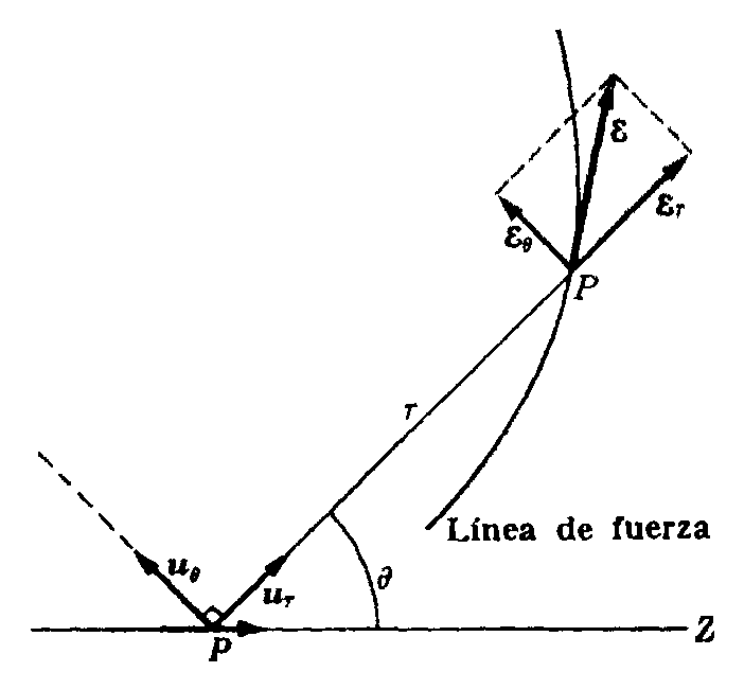
\includegraphics[width=.5\textwidth]{imagenes/imagenes24/T24IM03.png}
\end{figure}
\begin{figure}[H]
	\centering
	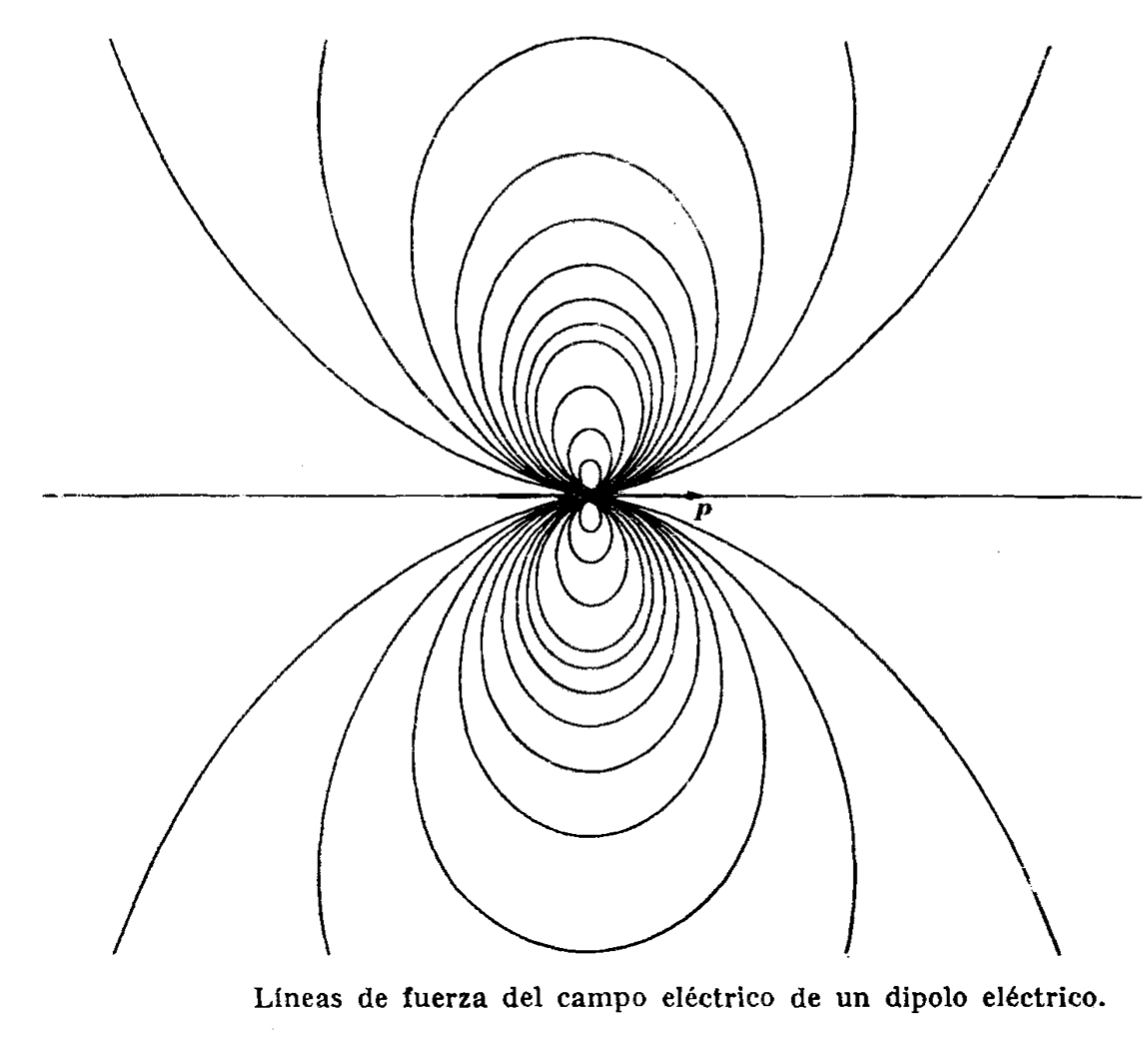
\includegraphics[width=.5\textwidth]{imagenes/imagenes24/T24IM04.png}
\end{figure}
\end{multicols}
El hecho de que las dos carda estén separadas una pequeña distancia $a$ hace que el campo eléctrico no sea nulo.

Definimos el \emph{momento dipolar de una agrupación de cargas} como 

$\displaystyle \vec p= q_1 \vec r_1+ q_2 \vec r_2+ \cdots + q_N \vec r_N = \sum_{i=1}^N q_i \vec r_i$

Si elegimos como dirección de $\vec p$ la del eje $z$, podremos escribir: 

$p=\sum q_iz_i=\sum q_ir_i \cos \theta_i$ 


Como va a reaccionar la materia:

La materia está compuesta por átomos o moléculas que, en general, son neutras eléctricamente. Pero, ?`qué ocurre cuando se aplica un campo eléctrico externo? El átomo se distorsionará y esa configuración instantánea la podemos considerar como un dipolo.

\begin{figure}[H]
	\centering
	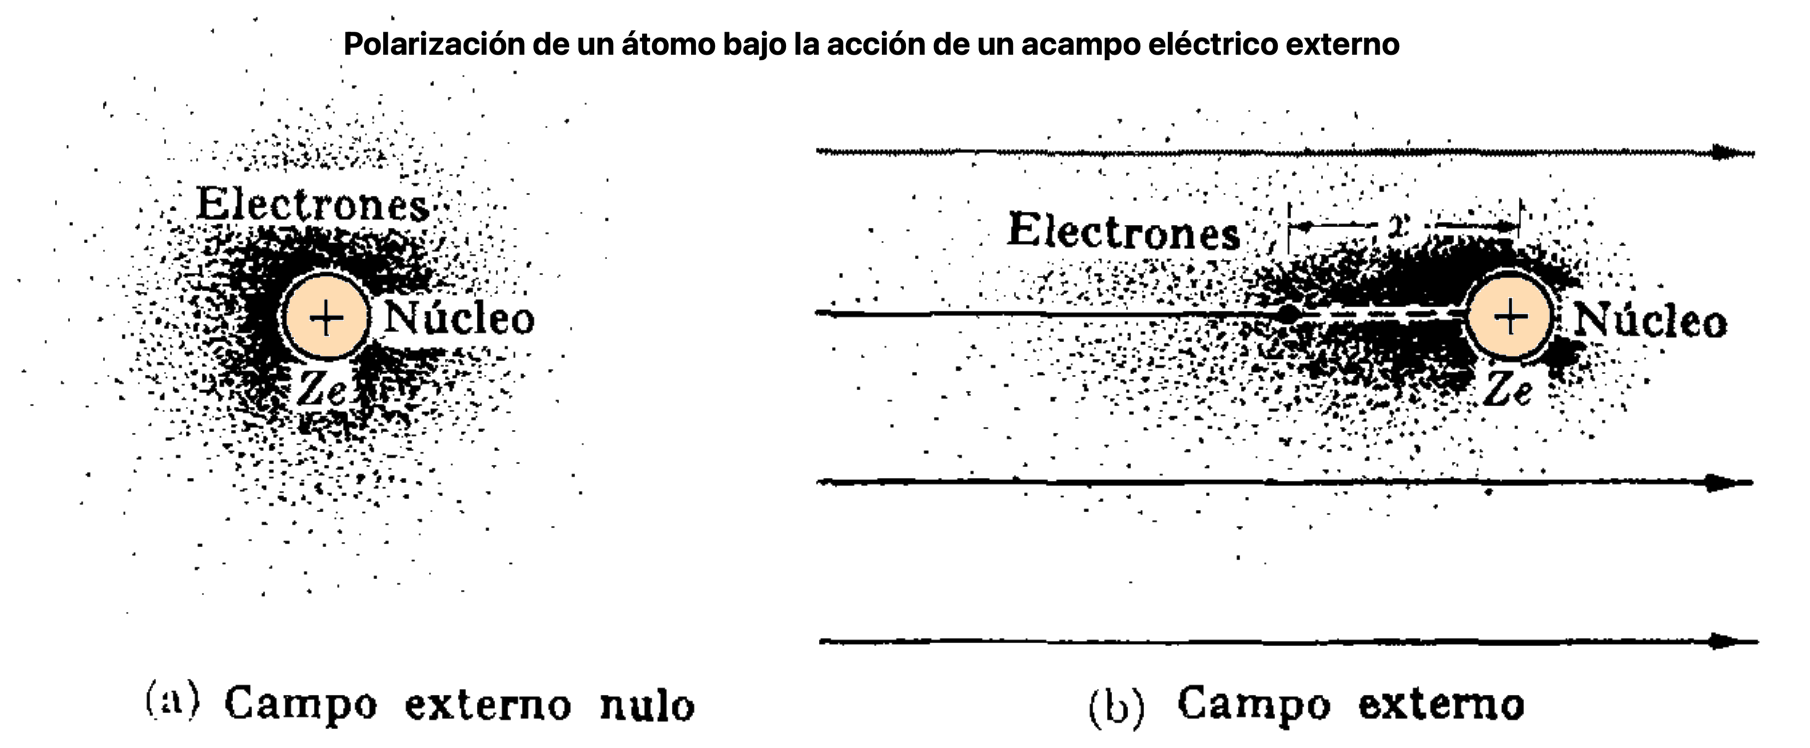
\includegraphics[width=1\textwidth]{imagenes/imagenes24/T24IM05.png}
\end{figure}

Existen moléculas que, en valor medio, presentan momentos dipolares, $HCl$, son las llamadas \emph{moléculas polares}.

\emph{Dipolos inducidos}: son aquellos que se inducen por la presencia de campos eléctricos externos.

Cuando un dipolo eléctrico se coloca en un campo eléctrico, se produce una fuerza sobre cada carga del dipolo, la resultante de estas fuerzas es $\vec F=-q\vec E + q \vec E'=q(\vec E'-\vec E)$

Si el dipolo está orientado en la dirección del campo y éste lo está en la dirección del eje $x$, entonces $E'-E=\displaystyle \dv{E}{x} \dd x=\dv{E}{x} a \to F=p\dv{E}{x}$.

Un dipolo eléctrico paralelo al campo eléctrico tiende a moverse en la dirección en que el campo crece.

Veamos cual es la energía potencial que tiene un dipolo en presencia de un campo eléctrico externo.

$\displaystyle \mathcal E_p=qV-qV'=q(V-V')=q\dv{V}{x}\dd x=q\dv{V}{x} a=\dv{V}{x}$

Como $E=\displaystyle -\dv{V}{x} \ \to \ \mathcal E_p=-pE$

\begin{multicols}{2}
Como el campo eléctrico es (central) conservativo, según el teorema de Lejeune-Dirichlet, todo sistema físico en un campo conservativo 

En tres dimensiones: 

$\mathcal E_p=-\vec p \cdot \vec E=-pE\cos \theta$. 

Para $\mathcal E_p$ mínima $\to \theta=0$, luego $\vec p \ || \ \vec E$. \emph{El dipolo eléctrico tiende a alinearse en la dirección del campo}.

Aparece un par de fuerzas de momento $\vec M=\vec a \times q\vec E=\vec p \times \vec E$ que hace girar al dipolo y cesará cuando sean paralelos.

\begin{figure}[H]
	\centering
	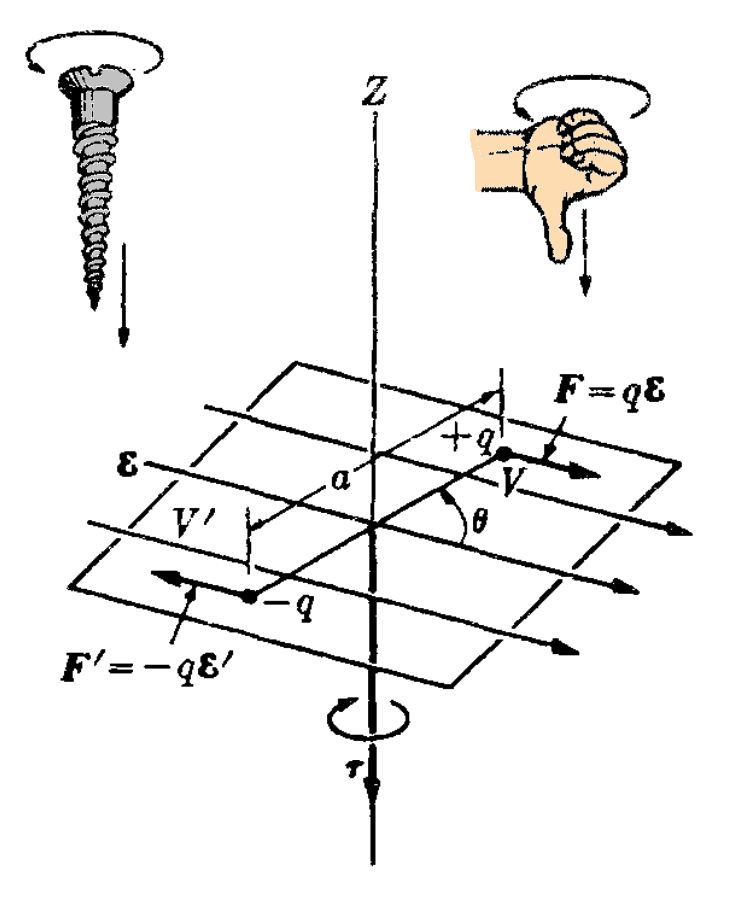
\includegraphics[width=.55\textwidth]{imagenes/imagenes24/T24IM06.png}
\end{figure}
\end{multicols}

\section{Polarización de la materia}


\begin{multicols}{2}
Cuando una porción de materia se coloca bajo la acción de un campo eléctrico, la materia tiende a orientar sus dipolos en la dirección del campo. 

Este fenómeno recibe el nombre de \emph{polarización de la materia} y, cuando ocurre, se dice que la materia se ha polarizado.
\begin{figure}[H]
	\centering
	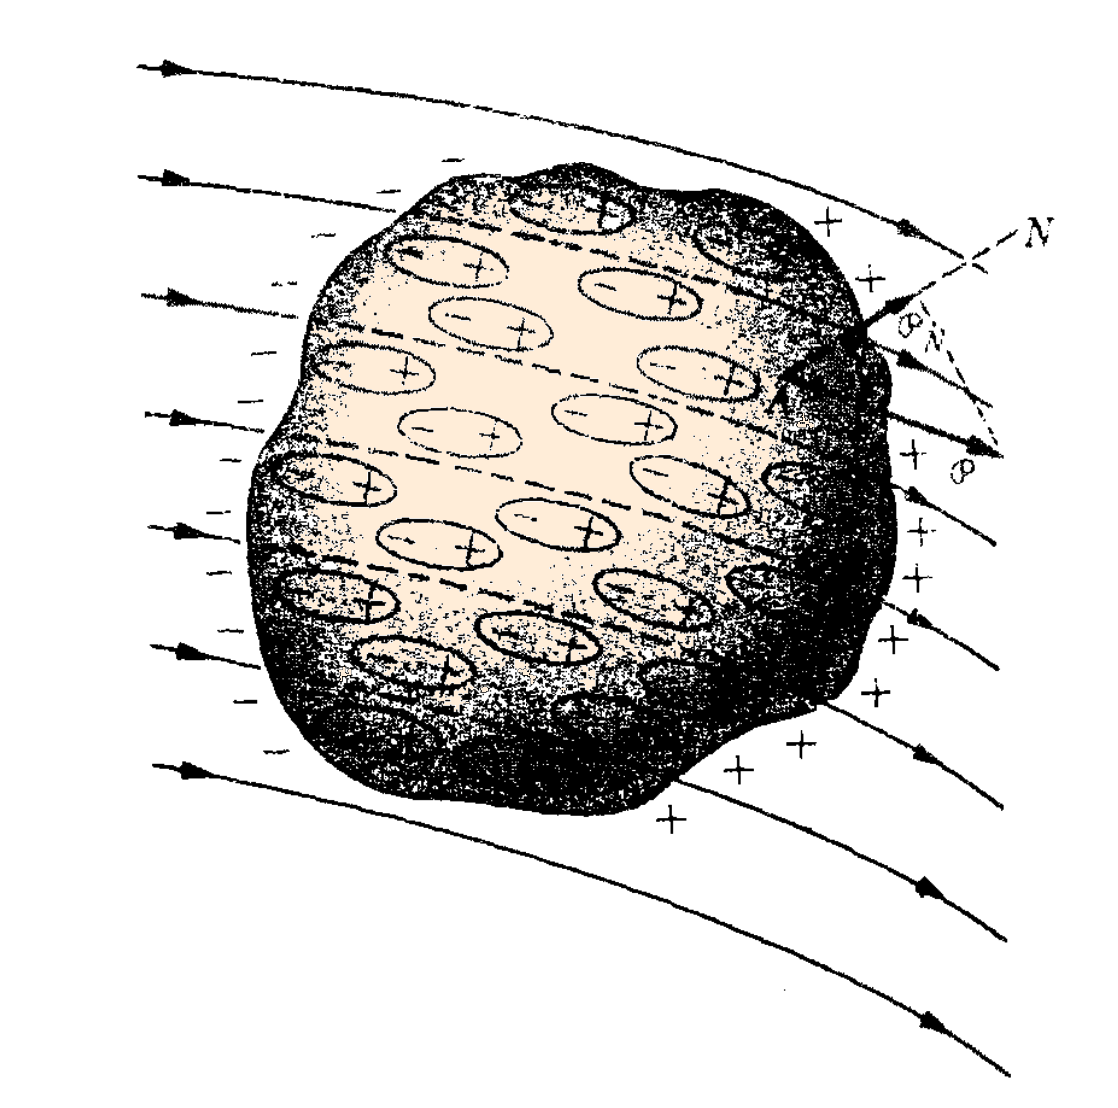
\includegraphics[width=.5\textwidth]{imagenes/imagenes24/T24IM07.png}
\end{figure}
\end{multicols}

Cuando un material se puede polarizar por el efecto de un campo eléctrico exterior se dice que es un \emph{\textbf{dieléctrico}}. Podemos interpretar esa porción polarizada de la materia como un gran dipolo.

Se define una nueva magnitud llamada \emph{polarización} de un material, $\overrightarrow{\mathcal P}$, como el momento dipolar por unidad de volumen de la muestra.

\begin{equation}
	\overrightarrow{\mathcal P} \ = \ \dv{\vec p}{\tau}
\end{equation}

Si la muestra es homogénea, cada átomo o molécula tendrá su momento dipolar $\vec p$ y, si hay $n$ átomos o moléculas por unidad de volumen, $\overrightarrow{\mathcal P}=n\vec p$.

Como $\vec p=q\vec a$, en el $SI$ de unidades, $\overrightarrow{\mathcal P}$ se expresa como $\mathrm{C\ m}^{-2}$. Como también en el $I$ ocurre que $\varepsilon_0 \vec E$ se expresa en $\mathrm{C\ m}^{-2}$, se puede concluir que ya que el material se polariza debido a la existencia de un campo exterior $\vec E$, la polarización ha de ser proporcional a éste, $\varepsilon_0 \vec E$, por lo que:

\begin{equation}
	\overrightarrow{\mathcal P}\ = \ \chi_e \ \varepsilon_0 \ \vec E
\end{equation}

$\chi_e$ es la \emph{\textbf{susceptibilidad eléctrica}}, un número adimensional, y positivo.

\begin{multicols}{2}
$\vec E \ \bot \ \vec S; \quad \displaystyle \int \dd \vec p = \int_\tau \overrightarrow{\mathcal P} \dd \tau$

$\vec p_{total}=\overrightarrow{\mathcal P} \tau=\overrightarrow{\mathcal P} S l=(\overrightarrow{\mathcal P} S)\ l$

Comparando con la definición de dipolo eléctrico, $\vec p=q\vec a$,
deducimos que el material se comportará cono un \emph{gran dipolo} de carga $q=\mathcal P S$ por lo que podemos asimilar $\mathcal P=\sigma$, densidad superficial de carga que se induce en el dieléctrico cuando se le somete a un campo eléctrico externo.

\begin{figure}[H]
	\centering
	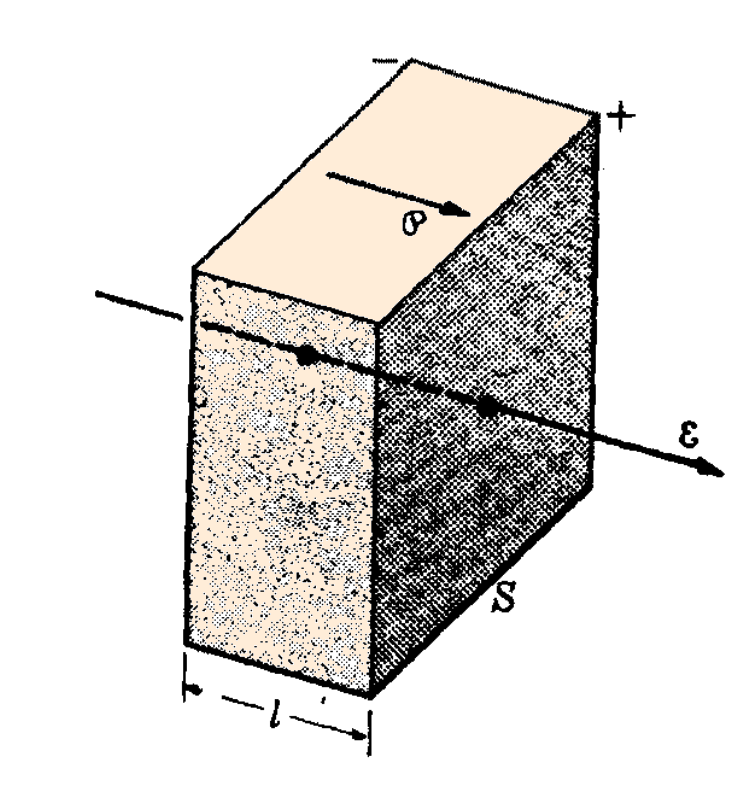
\includegraphics[width=.55\textwidth]{imagenes/imagenes24/T24IM08.png}
\end{figure}
\end{multicols}


Aunque este resultado se ha obtenido para una disposición geométrica particular, tiene validez general, y \emph{la carga por unidad de área sobre la superficie de una porción de materia polarizada es igual a la componente de la polarización $\mathcal P$ en la dirección de la normal a la superficie del cuerpo}.


Veamos como reacciona un material conductor, un metal. 

Los metales se caracterizan por que tienen cargas libres, electrones. Cuando se les somete a un campo eléctrico externo hay un reordenamiento electrónico de forma que el campo eléctrico en el interior sea cero $(\vec E^{(i)})$ y el campo eléctrico en la superficie debe ser normal, ya que si tuviera una componente paralela, las cargas se moverían sobre la superficie del conductor. Así, el conductor alcanza el equilibrio eléctrico.

--- Si $\vec E^{(i)}=0 =\vec \grad V^{(i)}\ \to \ V^{(i)}=cte$ y, además, 

--- $\vec \grad \cdot \vec E^{(i)}=0=\dfrac {\rho^{(i)}}{\varepsilon_0}=0 \ \to \ \rho^{(i)}=0$ 

\emph\textbf{{Toda la carga eléctrica de un conductor en equilibrio está sobre su superficie}}.\footnote{Campana de Gauss.}



\begin{multicols}{2}
Cálculo del $\vec E$ en las proximidades de la superficie de un metal, para ello, tomamos superficie gaussiana el tubo de la figura.

En el interior $\vec E^{(i)}=0$, en la superficie, el $\vec E \ || \ \vec S$, por lo que solo hay flujo en la superficie exterior del metal.

$\displaystyle \int_S \vec E \cdot \dd \vec S =ES=\dfrac{\sigma S}{\varepsilon_0}$

EN el exterior: $ \ E=\dfrac \sigma {\varepsilon_0}$

\begin{figure}[H]
	\centering
	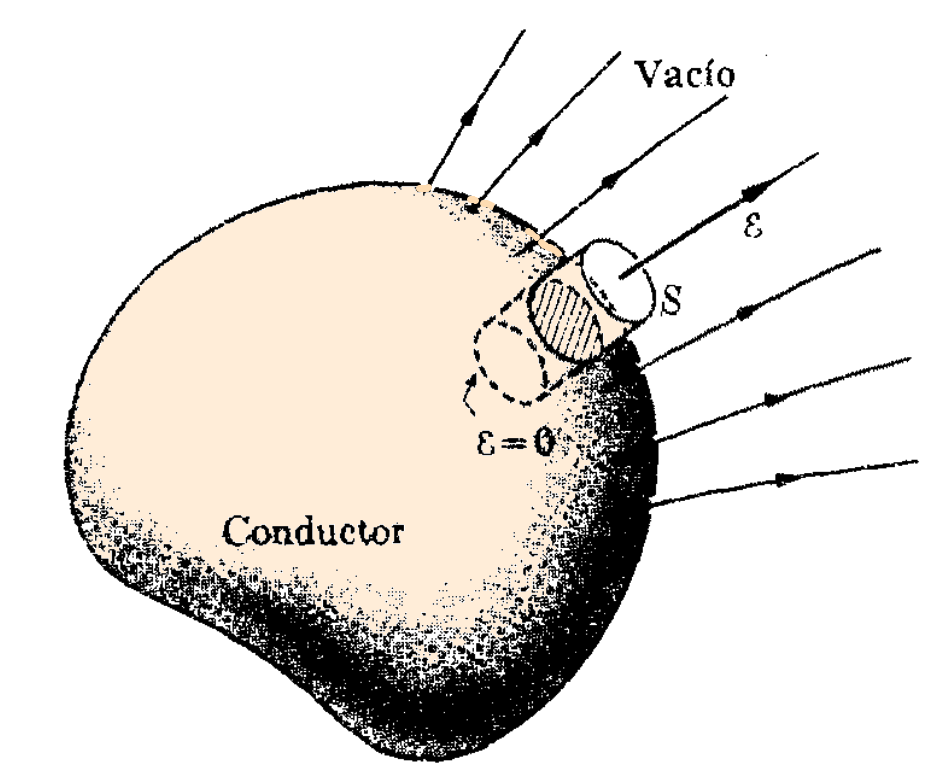
\includegraphics[width=.55\textwidth]{imagenes/imagenes24/T24IM09.png}
\end{figure}
\end{multicols}
Conclusión: en un dieléctrico, las cargas que se inducen están congeladas, no se mueven en el seno del material; en los metales las cargas sí se mueven, reciben el nombre de \emph{cargas libres}.

\section{Desplazamiento eléctrico}

\begin{multicols}{2}
	Dieléctrico colocado entre placas metálicas con cargas opuestas. Las cargas de las placas son cargas libres y las cargas de la superficie del dieléctrico son cargas de polarización.

$\sigma_{libre}$, densidad superficial de carga sobre el metal, coincide, en esta distribución geométrica, con el módulo del vector polarización $\vec {\mathcal P}$, que llevará la misma dirección y sentido que el campo eléctrico.
\begin{figure}[H]
	\centering
	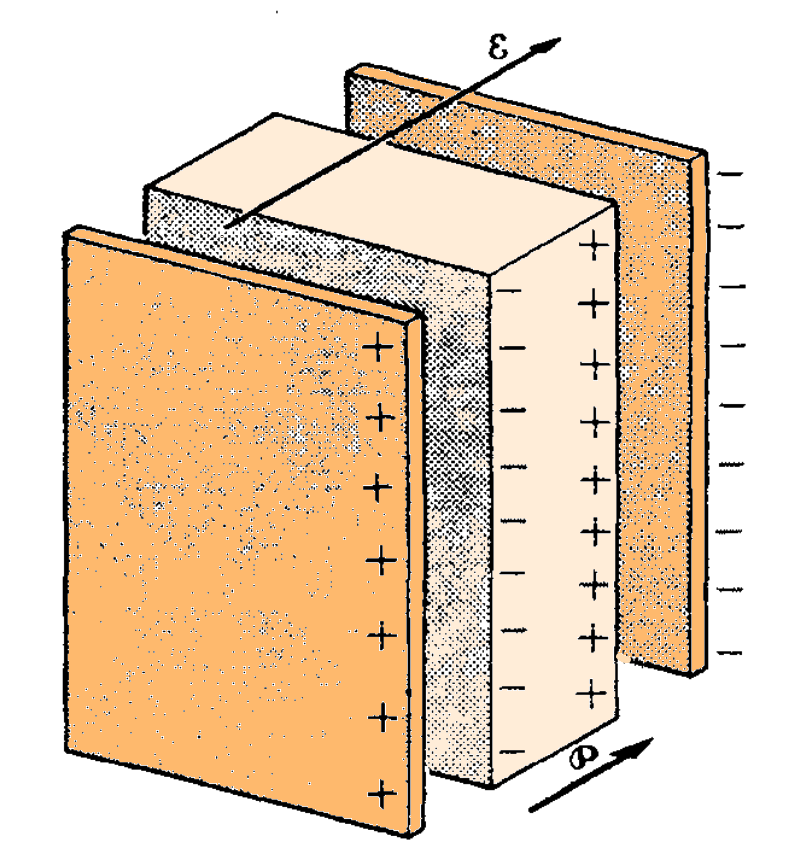
\includegraphics[width=.5\textwidth]{imagenes/imagenes24/T24IM10.png}
\end{figure}
\end{multicols}

Calculemos el campo eléctrico en el interior del dieléctrico, para ello, recordamos que el campo eléctrico que existe entre dos placas metálicas plano paralelas cargadas vale: $\vec E=\sigma / \varepsilon_0$.

En nuestro caso: $\ E=\dfrac{\sigma_{neta}}{\varepsilon_0}=\dfrac{\sigma_{libre}- \mathcal P}{\varepsilon_0} \ \ \to \ \  \boldsymbol{ \sigma_{libre}=\varepsilon_0 E + \mathcal P }$

Es expresión que da las cargas libres sobre la superficie de un conductor rodeado por un dieléctrico en función del campo eléctrico en el dieléctrico y de la polarizacíón del mismo

Observamos que, en el caso que estamos estudiando, $E$ y $\mathcal P$ son vectores en la misma dirección, los resultados anteriores sugieren la conveniencia de introducir un nuevo vector, llamado \emph{\textbf{desplazamiento eléctrico}}, definido por

$\vec{\mathcal D}=\varepsilon_0 E + \vec{\mathcal P}=\mathcal D \vec u_N;\qquad \mathcal D=\sigma_{libre};\qquad \vec {\mathcal P} \cdot \vec u_N=\sigma_{libre}$

Es decir, la componente de $\mathcal D$ según la normal a la superficie de un conductor sumergido en un dieléctrico da la densidad de carga superficial en el conductor.

De otra forma: $\quad  \vec{\mathcal D}=\varepsilon_0 \vec E + \chi_e \varepsilon_0 \vec E = \boldsymbol{\varepsilon_0 (1+\chi_e)} \vec E =\boldsymbol{\varepsilon} \vec E$

$$\subrayado{ \ \boldsymbol{
\vec{\mathcal D}\ = \ \varepsilon \ \vec E \qquad  \varepsilon \ = \ \varepsilon_0 \ (1+\chi_e) \qquad \varepsilon:\ \textbf{permitividad del medio} }
\ } $$


Definimos $\ \varepsilon'=\dfrac{\varepsilon}{\varepsilon_0}=1+\chi_e$ es la \emph{constante dieléctrica del medio o permitividad relativa.}

Calculemos, ahora, el flujo del vector desplazamiento eléctrico.

$\displaystyle \boldsymbol{\Phi_{\mathcal D}=}\oint_S \vec{\mathcal D} \cdot \dd \vec S = \oint_S \varepsilon \vec E \cdot \dd \vec S = \varepsilon \oint_S \vec E \cdot \dd \vec S \boldsymbol{=\varepsilon \Phi_E}$

$\vec{\mathcal D}\cdot \vec u = \sigma_{libre}; \ \ \dd \vec S = \vec u \ \dd S; \qquad \displaystyle \oint_S \sigma_{libre} \dd S = q_{libre}$

por lo que

\begin{equation}
\subrayado{ \boldsymbol{
\Phi_E \ = \ \oint_S \vec E \cdot \dd \vec S\ = \ \dfrac {q_{libre}}{\varepsilon}
} \ }	
\end{equation}

Comparando leste resultado con la ley de Gaus vemos que el efecto del dieléctrico sobre el campo eléctrico $E$ es reemplazar $\varepsilon_0$ por $\varepsilon$ si sólo se consideran las cargas libres. Por consiguiente, la fuerza, el campo y el potencial eléctricos producidos por una carga puntual inmersa en un dieléctrico serán:

\begin{equation}
\subrayado{ \ \boldsymbol{
\vec F=\dfrac {q_1\ q_2}{4\pi \varepsilon r^2} \ \vec u_r	; \qquad \quad \vec E= \dfrac {q} {4\pi \varepsilon r^2} \ \vec u_r; \quad \qquad V= \dfrac {q} {4\pi \varepsilon r} } \ }
\end{equation}

Por lo general, $\varepsilon>\varepsilon_0$, por lo que \emph{la interacción eléctrica entre dos cuerpos  es de menor intensidad  cuando en vez de producirse en el vacío se produce en un medio dieléctrico.}

\section{Capacidad. Condensadores.}

$\varepsilon$, permitividad de cualquier medio dieléctrico.

$\vec E=\dfrac {q} {4\pi \varepsilon r^2} \ \vec u_r=-\vec {\grad} V; \qquad V=\dfrac {q} {4\pi \varepsilon r} $

En una superficie esférica: $V=\dfrac {q} {4\pi \varepsilon R} \ \to \ 4 \pi \varepsilon R= \dfrac q V$ , $q$ es la carga sobre la esfera y $V$ el potencial eléctrico en la superficie de la esfera.

Para una esfera rodeada de un medio dieléctrico determinado, $4\pi \varepsilon R=cte$, por lo que $\dfrac q V =cte$ en estos casos.

Llamamos \emph{capacidad}, $\boldsymbol{ C=}4\pi \varepsilon R=\boldsymbol{ \dfrac q V}$.  En el sistema internacional de unidades, la capacidad se mide en \emph{farad}\footnote{El farad o faradio recibe su nombre en honor al físico británico Michael Faraday (1791-1876)}, $\mathrm {C \ V}=F$.

$1 \mu\mathrm{F} = 10^{-6} \ \mathrm{F}; \quad 1 n\mathrm{F}=10^{-9} \ \mathrm{F}; \quad 1 p\mathrm{F}=10^{-12} \ \mathrm{F}$

\begin{multicols}{2}
Supongamos dos conductores cargados con cargas $+Q$ y $-Q$.

Llamamos capacidad de ese sistema de dos conductores a la relación que liga la carga de uno de ellos, en valor absoluto,  con la diferencia de potenciales, también en valor absoluto.

$$C\ = \ \dfrac{Q}{v_2-v_1} \ = \ \dfrac Q V$$
\begin{figure}[H]
	\centering
	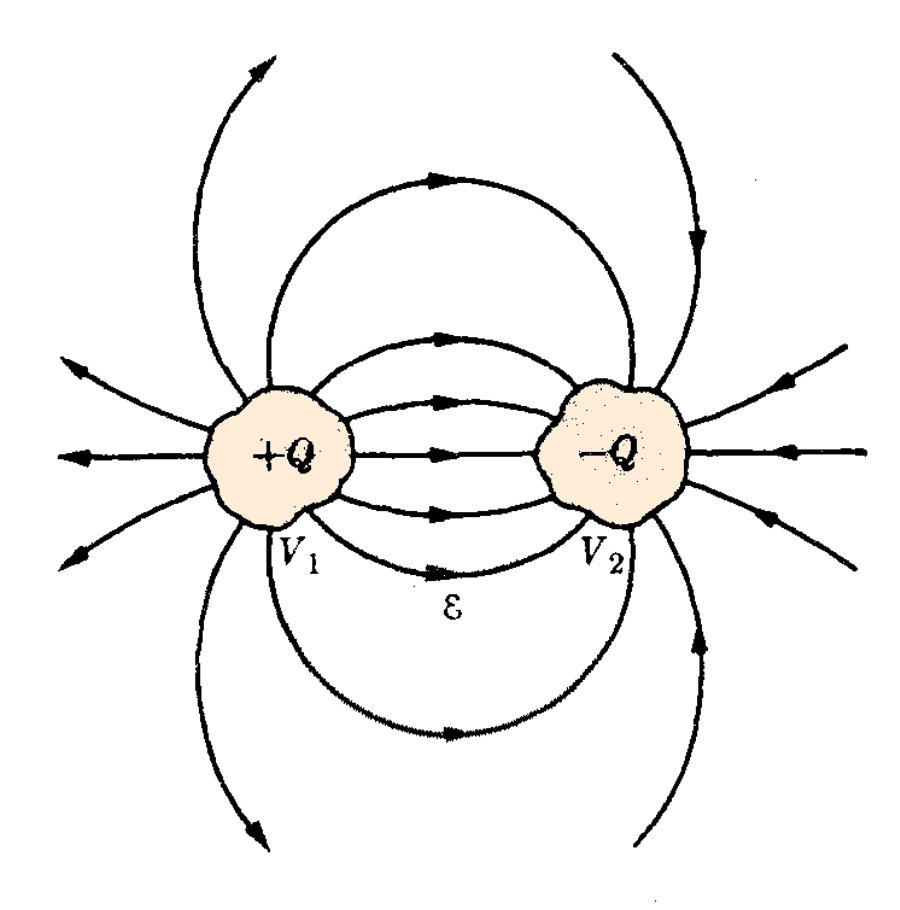
\includegraphics[width=.45\textwidth]{imagenes/imagenes24/T24IM11.png}
\end{figure}	
\end{multicols}

\begin{multicols}{2}
	Calculemos la capacidad de un conductor de caras planoparalelas.

$E=\dfrac{V_2-V_1}{d}; \quad E=\dfrac \sigma E$

$C=\dfrac {Q}{V_2-V_1}=\dfrac{\sigma_{libre}S}{Ed}=\dfrac{\varepsilon E S}{E d}$

$C=\dfrac{\varepsilon S}{d}$

La capacidad solo depende del medio y de las características geométricas del conductor.
\begin{figure}[H]
	\centering
	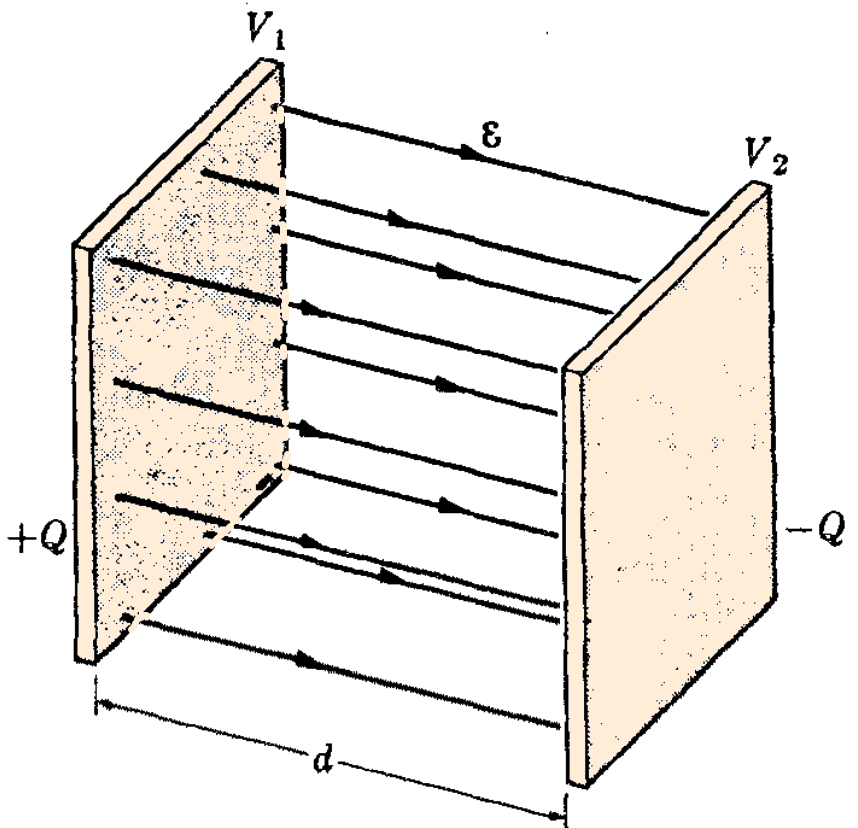
\includegraphics[width=.45\textwidth]{imagenes/imagenes24/T24IM12.png}
\end{figure}
\end{multicols}

La representación esquemática de un condensador es ---||---

La capacidad de un condensador en el vacío es $C=\dfrac {\varepsilon_0 S}{d}$; en un medio dieléctrico $C=\dfrac Q V=\dfrac{\varepsilon S}{d}$, lo que nos permite calcular la permitividad relativa $\varepsilon'$ del medio.

\section{Combinación de condensadores}

Los condensadores pueden en dos formas, \emph{serie o paralelo}.

En la combinación en serie , la placa negativa de un condensador se conecta a la positiva del próximo, y así sucesivamente. En consecuencia todos los condensadores tienen la misma carga, positiva o negativa, sobre sus placas.

En la asociación paralelo, todas las placas positivas se conectan a un punto común, y las negativas también a otro punto común, de modo que la diferencia de potencial es la misma para todos los condensadores.

\begin{figure}[H]
	\centering
	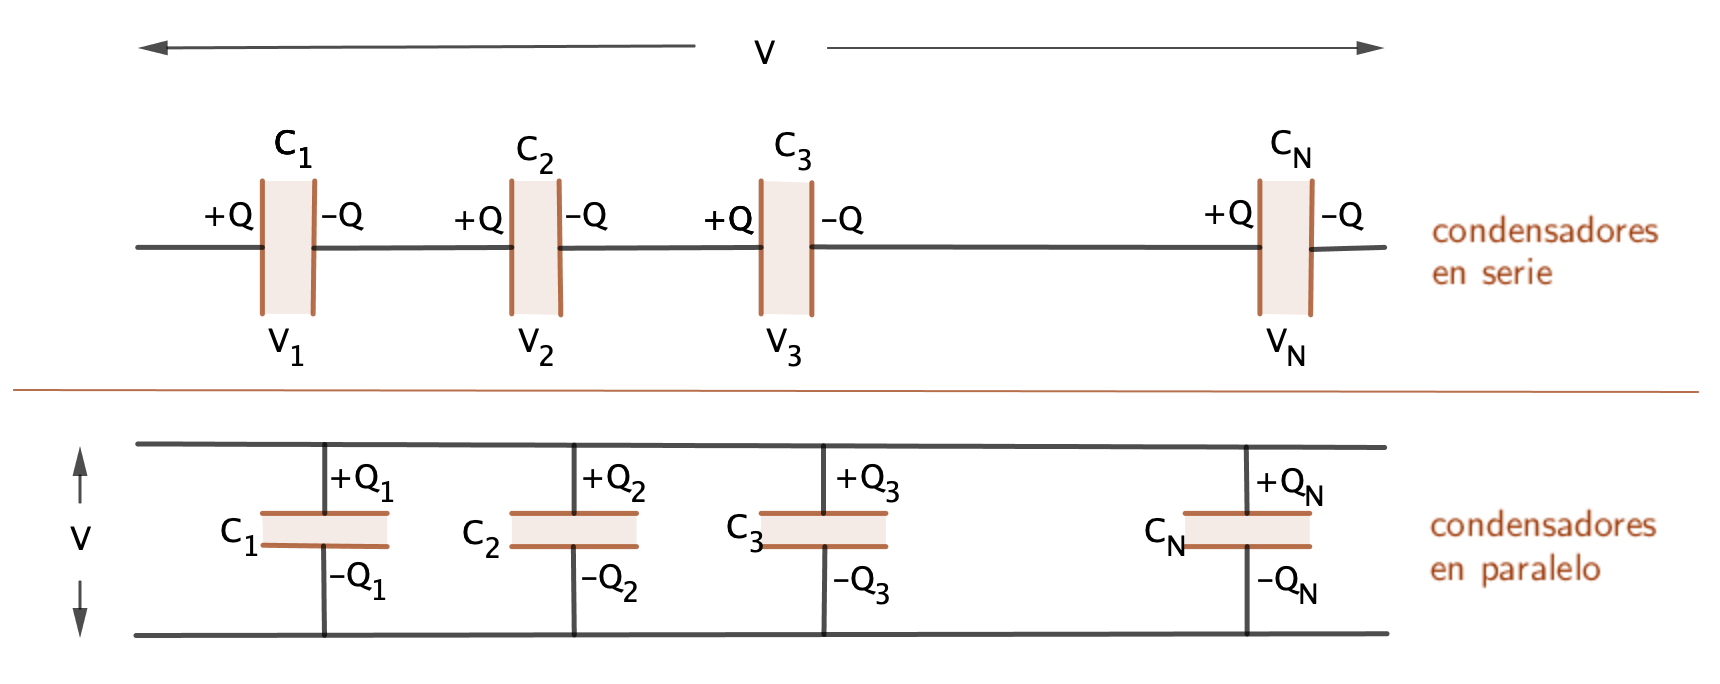
\includegraphics[width=1\textwidth]{imagenes/imagenes24/T24IM14.png}
\end{figure}

\textbf{Condensadores en serie.}

$V_i$ es la diferencia de potencial entre las placas del condensador $i$; $q_i$ carga en el condensador $i$; $q_{i+1}-q_i=0$, puesto que la carga no atraviesa el dieléctrico.

$V=V_1+V_2+\cdots +V_N=\displaystyle \sum_{i=1}^N V_i= \dfrac {q_1}{C_1}+ \dfrac {q_2}{C_2}+ \cdots +  \dfrac {q_N}{C_N}$

Como $q_{i+1}-q_i=0 \ \to \ q_{i+1}=q_i=q$

$\displaystyle V=  q \left( \dfrac 1 {C_1}+\dfrac 1 {C_2}+\cdots +\dfrac 1 {C_N} \right) = q \sum_{i=1}^N \dfrac 1 {C_i}$

$\displaystyle V= q \sum_{i=1}^N \dfrac 1 {C_i} \quad \dfrac V q = \dfrac 1 C = \sum_{i=1}^N \dfrac 1 {C_i}$

Capacidad total de un sistema de condensadores en serie:

\begin{equation}
\subrayado{\ \boxed{\ \boldsymbol{ \dfrac 1 C \ = \  \sum_{i=1}^N \dfrac 1 {C_i} } \ } \ }	
\end{equation}


\textbf{Condensadores en paralelo.}

Ahora ya no tiene que ser la misma la $q$ en los condensadores porque no hay polarización como en el caso anterior.

$q_1=C_1\ V; \ q_2=C_2\ V; \ \cdots \ q_N=C_N\ V$, sumando,

$Q=q_1+q_2+ \cdots + q_N=V(C_1+C_2+ \cdots + C_N)=V\ C$, por lo que

\begin{equation}
\subrayado{\ \boxed{\ \boldsymbol{ C\ = \ \sum_{i=1}^N C_i} \ } \ }	
\end{equation}

\begin{figure}[H]
	\centering
	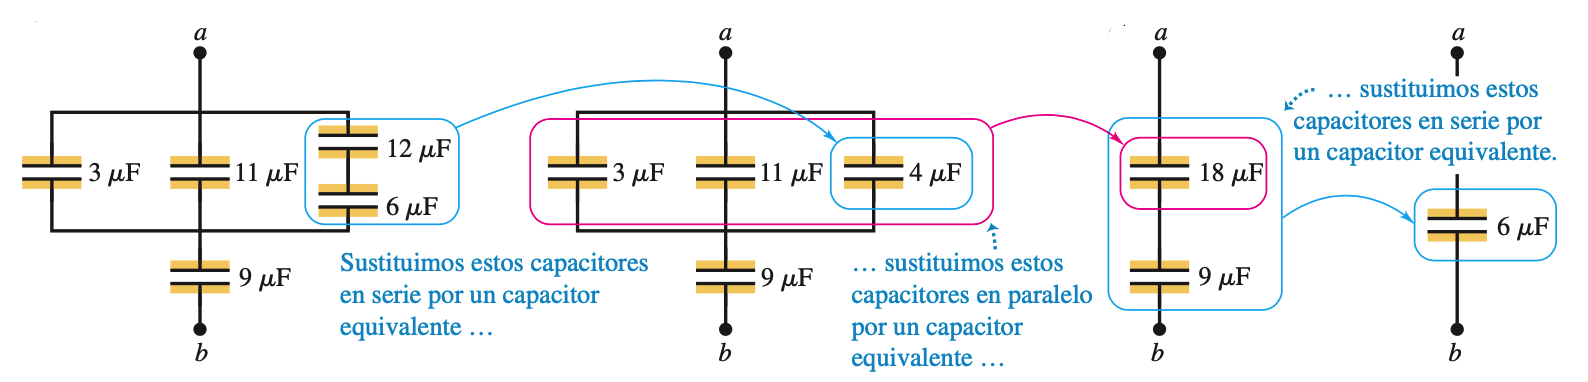
\includegraphics[width=1\textwidth]{imagenes/imagenes24/T24IM17.png}
\end{figure}

\section{Energía del campo eléctrico}

Para cargar un conductor es necesario gastar energía porque, para suministrarle más carga, debe realizarse trabajo para vencer la repulsión de las cargas ya presentes. Este trabajo ocasiona un aumento en la energía del conductor

Consideremos un conductor de capacidad $C=q/V$ y vamos a añadirle una carga $\dd q$ que traemos desde el infinito, tendrá que vencer la repulsión del campo eléctrico debido a la carga que hemos depositado en el conductor para lo que deberá consumir energía.

$\dd \mathcal E_p=V\ \dd q = \dfrac q C \ \dd q \quad \to \quad \displaystyle \mathcal E_p=\int_0^Q \dfrac q C \dd q$

El trabajo necesario para cargar un conductor es igual a la variación de la energía potencial ya que el campo eléctrico es conservativo.

\begin{equation}
\subrayado{ \ \boxed{ \ \boldsymbol{ \mathcal E_p\ = \  \dfrac 1 2 \ \dfrac {Q^2} C } \ } \ }	
\end{equation}

Para el caso particular de un metal de simetría esférica, $C=4\pi \epsilon R$, tendremos que
\begin{equation}
\subrayado{ \ \boxed{ \ \boldsymbol{ \mathcal E_p\ = \  \dfrac 1 2 \ \dfrac {Q^2} {4\pi \varepsilon R} } \ } \ }	 \qquad \textbf {conductor esferico}
\end{equation} 

\emph{Interpretación física}: En valor absoluto, $\vec E=\dfrac{Q}{4\pi \varepsilon r^2}$, con $r>R$ puesto que en el metal la carga se distribuye sobre la superficie.

Calculemos la integral $\displaystyle \int_R^\infty E^2 \dd \tau=\int_R^\infty \dfrac {Q^2}{(4\pi \varepsilon^2 r^2)^2} 4 \pi r^2 \dd r$, es decir

$\displaystyle \int_R^\infty E^2 \dd r=\dfrac {Q^2}{4\pi \varepsilon^2 R}$, comparando con la expresión de la energía potencial del conductor esférico,
$\displaystyle \mathcal E_p \ = \ \dfrac 1 2 \ \varepsilon \int_{\text{todo el espacio}} E^2 \ \dd \tau$

A esta expresión se le puede dar una interpretación física importante. Podemos decir que la energía utilizada en disponer las cargas se ha almacenado en el espacio que las rodea, de modo que al volumen $\dd \tau$ corresponde la energía $\frac 1 2 \varepsilon E^2 \dd \tau$. Por consiguiente la energía por unidad de volumen, o \emph{densidad de energía} $e_E$ `almacenada' en el campo eléctrico es

\begin{equation}
\boldsymbol{ e_E\ = \ \displaystyle \dv{\mathcal E_p}{\tau}\ = \ \dfrac 1 2 \ \varepsilon \ E^2  } 	
\end{equation}

Esta interpretación de la energía de un sistema de partículas cargadas distribuidas en todo el espacio donde existe el campo eléctrico es muy útil en la discusión de muchos procesos.

\section{Problemas}

\begin{prob}
Un condensador de armaduras paralelas tiene una capacidad de $100\ p \mathrm{F}$	y el área de us placas es de $100\ \mathrm{cm}^2$. Como dieléctrico tiene mica entre las placas, $\varepsilon'=5.4$. Para una diferencia de potencial de $100\ \mathrm{V}$, calcula el campo eléctrico en la mica, la carga libre en las placas y la carga superficial inducida en el dieléctrico.
\end{prob}

$\varepsilon=\varepsilon' \varepsilon_0=5.4 \cdot 8.854 \times 10^{-12}=2.78\times 10^{-11}  \ \mathrm{UI}$

$C=\varepsilon S/d \ \to \ d=\varepsilon S/C= 4.78\times 10^{-11} \cdot 10^{-2} / 10^{-10} = 4.78\times 10^{-3} \ \mathrm{m}$

$E=v/d=50/4.78\times 10^{-3}=1.046\times 10^4\ \mathrm{V m}^{-1}$

$E=\sigma_{libre}/\varepsilon \ \to \ \sigma_{libre}=\varepsilon E= 4.78\times 10^{-11} \cdot 1.046\times 10^4=5\times 10^{-7} \ \mathrm{C\ m}^{-2}$

$\sigma_{libre}=q_{libre}/S \ \to \ q_{libre}=5\times 10^{-7} \cdot 10^{-2}=5\times 10^{-9}\ \mathrm{C}$

$\sigma_{libre}=\varepsilon_0E+\mathcal P \ \to \ \mathcal P=\sigma_{libre}-\varepsilon_0E=0.5\times 10^{-7}-9.854\times 10^{-12}\cdot 1.046\times 10^4=4.07\times 10^{-7} \ \mathrm{C\ m}^{-2}$

$q_{ind}=\mathcal P S=\sigma_{ind}S=4.07\times 10^{-7} \cdot 10^{-2}=4.07\times 10^{-9} \ \mathrm{C}$

\begin{prob}
Un condensador tiene armaduras cuadradas de lado $a$ que forman un ángulo $\theta$ entre sí. Calcular la capacidad de este condensador para pequeños valores de $\theta$	
\end{prob}

$C=\dfrac {\varepsilon S}{d}; \quad \dd C=\dfrac {\varepsilon a x \dd x}{y}=\dfrac{\varepsilon a x \dd x}{l+x\tan \theta}$

Podemos considerar que estos condensadores elementales están conectados en paralelo: $C=\sum_i C_i$

\begin{figure}[H]
	\centering
	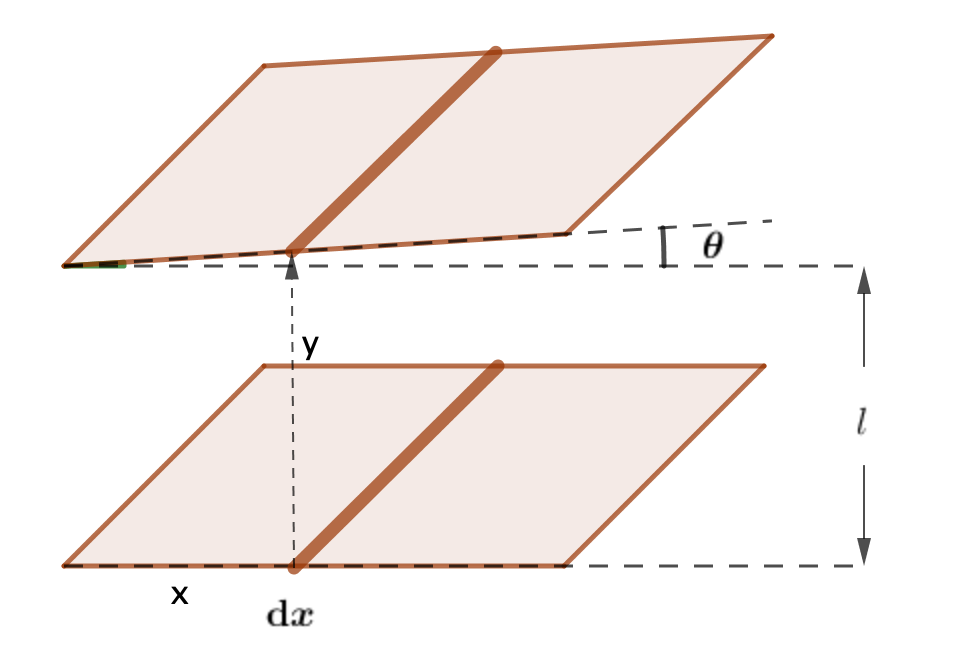
\includegraphics[width=.65\textwidth]{imagenes/imagenes24/T24IM18.png}
\end{figure}

$\displaystyle C=\int_0^a \dfrac{\varepsilon a x \dd x}{l+x\tan \theta}=\dfrac{\varepsilon a}{\tan \theta} \int_0^a \dfrac{\tan \theta  \dd x}{l+x\tan \theta} = \dfrac{\varepsilon a}{\tan \theta} \left[ \ln (l+x\tan \theta) \right]_0^a = \dfrac {\varepsilon a}{\tan \theta} [ \ln(l+a\tan \theta)-\ln l ]=\dfrac{\varepsilon a}{\tan \theta} \ln \left( 1+\dfrac{a \tan \theta}{l} \right) $

Para $\theta <<1 \ \to \ \tan \theta \approx \theta \ \to \ C\approx \dfrac{\varepsilon a}{\theta} \ln \left( 1+\dfrac{a \theta}{l} \right)$

Como $\ln(1+x) \approx x-\dfrac 1 2 x^2;\ \ x<<1$, McLaurin,

$C\approx \dfrac{\varepsilon a}{\theta} \left( \dfrac {a \theta}{l} - \dfrac 1 2 \dfrac {a^2 \theta^2}{l^2} \right)= \dfrac{\varepsilon a^2}{l} \left( 1 - \dfrac{a\theta}{2l} \right)$



\newpage %****************************************************

\begin{myblock}{La jaula de Faraday}
\vspace{2mm} Se conoce como jaula de Faraday al efecto por el cual campo eléctrico en el interior de un conductor en equilibrio es nulo, anulando el efecto de los campos externos. Esto se debe a que, cuando el conductor está sujeto a un campo eléctrico  externo, se polariza, de esta manera queda cargado positivamente en la dirección en que va el campo eléctrico , y cargado negativamente en el sentido contrario. Puesto que el conductor se ha polarizado, este genera un campo eléctrico igual en magnitud, pero opuesto en sentido al campo eléctrico , luego la suma de ambos campos dentro del conductor será igual a $0$.

\begin{figure}[H]
	\centering
	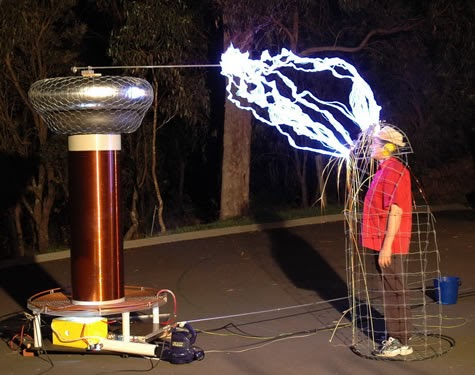
\includegraphics[width=.75\textwidth]{imagenes/imagenes24/T24IM16.png}
\end{figure}

\vspace{2mm} Se pone de manifiesto en numerosas situaciones cotidianas, por ejemplo, el mal funcionamiento de los teléfonos móviles en el interior de ascensores o edificios con estructura de rejilla de acero. Una manera de comprobarlo es con una radio sintonizada en una emisora de Onda Media. Al rodearla con un periódico, el sonido se escucha correctamente. Sin embargo, si se sustituye el periódico con un papel de aluminio, la radio deja de emitir sonidos: el aluminio es un conductor eléctrico y provoca el efecto jaula de Faraday.

\vspace{2mm} Este fenómeno, descubierto por Michael Faraday, tiene una aplicación importante en aviones o en la protección de equipos electrónicos delicados, tales como discos duros o repetidores de radio y televisión situados en cumbres de montañas y expuestos a las perturbaciones electromagnéticas causadas por las tormentas.
\end{myblock}



